% Generated by thesis/ch7/exp2/networks.py -- do not edit by hand.
\begin{sidewaysfigure}
  \centering
  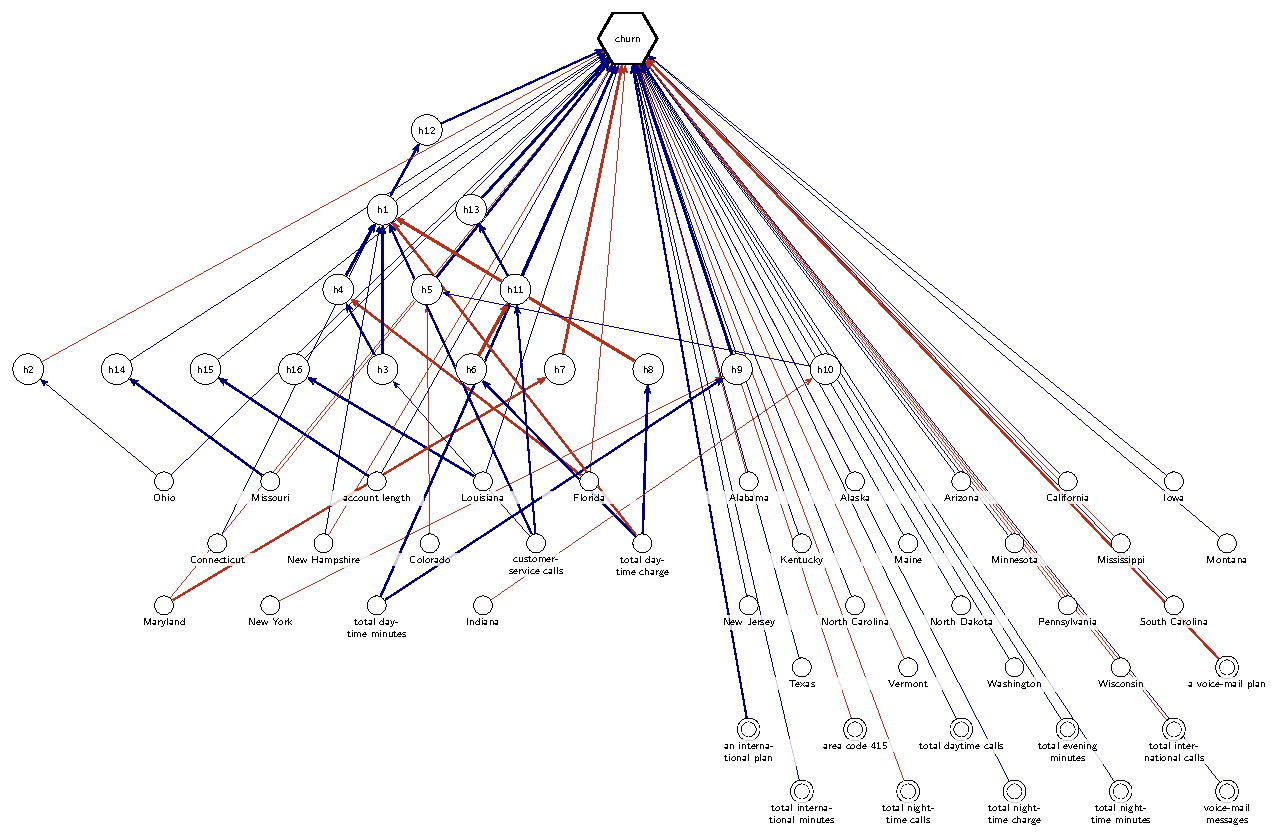
\includegraphics[width=\textheight,height=0.78\textwidth,keepaspectratio]{figures/exp2/networks/churn100-s5-raw}
  \caption{Churn, seed 5 (churn100-s5): the network as trained, before any explanation, in full. Inputs at the bottom (every input column its own node), hidden units by depth, the output at the top; 44 of 71 input columns are connected, with 16 hidden units and 75 enabled connections. Blue: positive weight (raises the score); red: negative weight (lowers it); thicker: larger weight. Orange outline and up arrow: raises the final prediction; teal and down arrow: lowers it; grey and double arrow: depends. Not used (no connection; 27 columns): Georgia, Hawaii, Idaho, Illinois, Kansas, Massachusetts, Arkansas, Michigan, Nebraska, New Mexico, Nevada, Oklahoma, Oregon, Rhode Island, South Dakota, Tennessee, Utah, Virginia, West Virginia, Wyoming, Washington DC, Delaware, area code 408, area code 510, total evening calls, total evening charge and total international charge.}
  \label{fig:exp2-net-churn100-s5-raw}
\end{sidewaysfigure}
